\documentclass{report}
\usepackage[utf8]{inputenc}
\usepackage[margin=1in]{geometry}
\usepackage{parskip}
\usepackage{setspace}
\linespread{1.5}
\usepackage{hyperref}
\usepackage{listings}

\usepackage{graphicx}
\DeclareGraphicsExtensions{.pdf,.png,.jpg,.tif}

\title{NST Physics and nbgrader}
\author{Niall McConville \\ PyCav Project}
\date{August 2016}

\begin{document}

\maketitle

\tableofcontents{}

\chapter{Introduction}
   nbgrader\footnote{\url{https://github.com/jupyter/nbgrader}} is a system which allows for the use of Jupyter\footnote{\url{http://jupyter.org/}} notebooks as a form of assessment material. 

Lecturers (or at least, their lackeys\footnote{\url{https://pycav.github.io/about/}}) can create a set of exercises contained within these notebooks. They can be distributed to students using the JupyterHub\footnote{\url{https://github.com/jupyterhub/jupyterhub}} server. 

From there, students can complete the computational exercises and return them (hopefully completed) to the lecturers. The lecturers can autograde the exercises and manually mark aspects which do not lend themselves easily to a machine marking them (such as graphs).

This document outlines how the PyCav project set up nbgrader for use within the Physics courses within the Natural Sciences Tripos.

Another source of documentation for nbgrader can be found here: \url{http://nbgrader.readthedocs.io/}.
   
\chapter{Setup}
    \section{JupyterHub}
    \subsection{Background}
    
        JupyterHub is a system which allows the hosting of a multi-user server which allows users to log in to and create Jupyter notebooks without hosting a server for themselves.
    
        Docker\footnote{\url{https://www.docker.com/}} is effectively a sandboxing system which allows JupyterHub to create single user Jupyter servers inside a set of isolated environments.
        
        The idea for this project was to set up an environment where students could experiment with Python without having to install any software locally. The above were selected as they were able to provide this environment.
        
    \subsection{Raven Authentication}
    
        All Cambridge students and staff have access to a crsid. This allows them to authenticate using the Raven\footnote{\url{https://raven.cam.ac.uk/}} service.
        
        To extend this functionality to JupyterHub, an authentication plugin jupyterhub-raven-auth\footnote{\url{https://github.com/PyCav/jupyterhub-raven-auth}} was written. It was used throughout the project.
        
    \subsection{Docker Configuration}
        
        The isolation provided by Docker is useful for running an assessment environment. It allows for caps to be placed on usage, especially in the instances of runaway code. Students are unable to view other student's files in a way that goes beyond setting access rights. It also allows for the simple addition of read only volumes, which we have exploited to share Demonstrations for everyone to see.
        
        Docker images are built from Dockerfiles (compare with Makefiles). These images are called by the Dockerspawner in the JupyterHub config. The Dockerspawner creates \textit{containers} which take up file space. It is possible to mount volumes in an NFS setup, using the \{username\} filter.
        
        In the Dockerfile provided below, one can see the extent of the customisation we provide. Notably, nbgrader is installed in each container.
        
        Docker containers (and their 'real' mounted volumes) should be continually backed up. We (as of \today) have not considered what the total size of such a system would be. For the 'Computational Models' course at Berkley, CA a 3 TB NFS was used for storage\footnote{\url{https://github.com/compmodels/jupyterhub-deploy}}.
        
        We have also set up the containers to execute the 'start-singleuser.sh' shell script. This contains code to create a new user, whose username matches the crsid of the individual logged into the JupyterHub. This is required as nbgrader will use this username in the filenames of submitted coursework.
        
        \clearpage
        
        Dockerfile:
        
        \lstinputlisting[frame=single]{setup/files/Dockerfile}
        
        \clearpage
       
        start-singleuser.sh file:
        
        \lstinputlisting[frame=single,language=Bash]{setup/files/start-singleuser.sh}
        \clearpage
    \subsection{The JupyterHub Config}
        \lstinputlisting[frame=single,language=Python]{setup/files/jupyterhub_config.py}
        
        \clearpage
    \section{nbgrader}

   \subsection{Background}
   
   nbgrader is a tool which allows for the assignment and grading of Jupyter notebooks. It can operate in numerous ways, the simplest of which is the manual distribution and collection of notebook assignments. The PyCav project uses a combination of nbgrader and JupyterHub to automate various aspects of the process.
   
   The documentation for nbgrader can be found here: \url{http://nbgrader.readthedocs.io/}.
   
   \subsection{Installation}
   
   The nbgrader was setup in two places,
   
   \begin{enumerate}
       \item The pycav server (the local server, where the JupyterHub is hosted).
       \item Within the Docker containers.
   \end{enumerate}

   The installation on the local server was for the utilisation of nbgrader's \textit{assign}, \textit{collect}, and \textit{formgrade} applications. These are to be run by the teaching staff, and will be discussed in a later chapter.
   
   The installation inside the Docker containers was for nbgrader's Jupyter extension, which calls nbgrader's \textit{fetch} and \textit{submit} applications. These will be run by the extension (and so not directly by students).
   
   Upon installation within a Docker image, a file called '.nbgrader.log' is created within the '/home/jovyan/work/' directory. As mentioned in the previous chapter, this \textit{must} have write access for the user or else the nbgrader functionality will not work.
   
   
   \subsection{Directory Structure}
   
   One can posit that there are effectively two sides to nbgrader directories: course directories and the distribution directory. These are both present on the local server.
   
   Central to the automation of distribution is the \textit{exchange} folder. Typically this is stored in the directory '/srv/nbgrader/exchange', although one can specify alternative directories. The exchange directory \textbf{must} be world readable and writable.
   
   Although any folder can be specified as the exchange folder, when mounting it to a Docker container, it is simplest to mount it to the container directory such that it appears as '/srv/nbgrader/exchange'. The default behaviour of nbgrader is to check this directory, with further (possibly complicated) configuration required to change this.
   
   Course directories provide a structure for the courses that can be provided. They will be elaborated upon in the next chapter.
   
   \subsection{JupyterHub Integration}
   
   \subsection{Teaching System Integration}
   
   Currently a work in progress. There will be a module which allows nbgrader to interface with the TiS.
    \section{Server}
        \begin{figure}[htb]
            \centering
            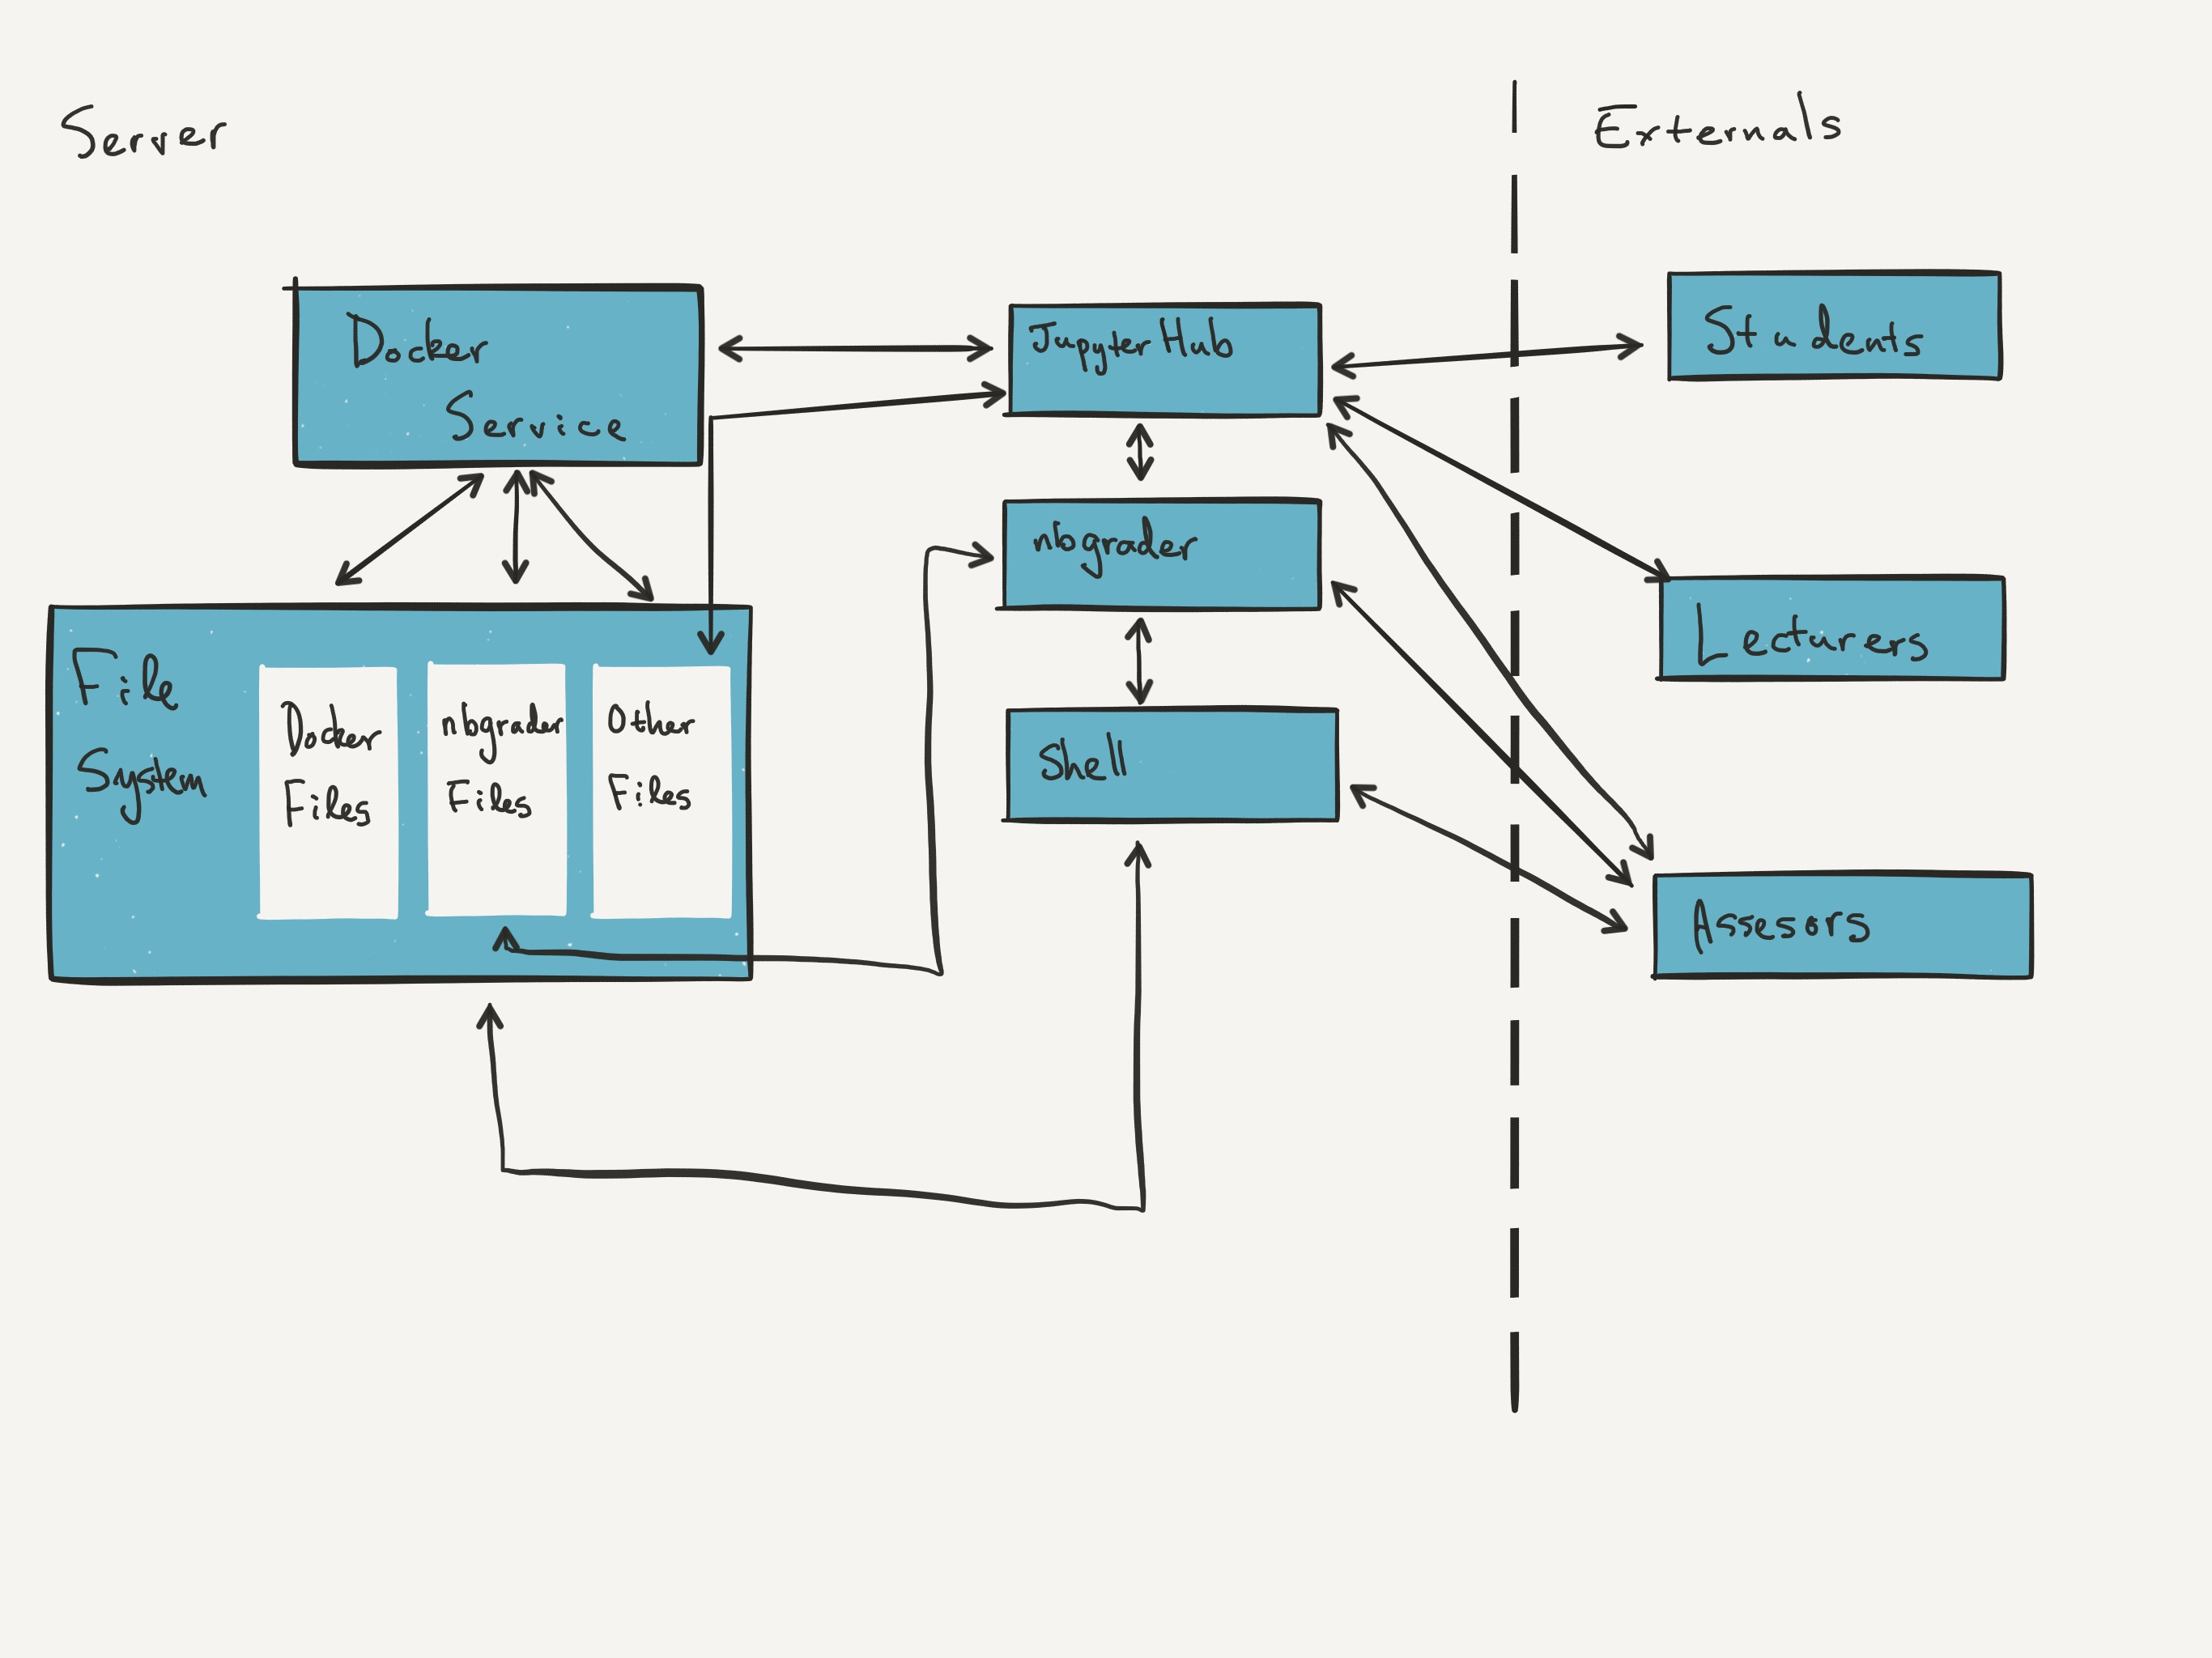
\includegraphics[width=0.9\linewidth]{setup/files/server_setup.png}
            \caption{The interactions between the various bits of software in relation to the users and the servers. Note that Assessors should be able to access software beyond the JupyterHub, for example, the nbgrader formgrade interface (which in turn relies on JupyterHub for authentication). Not depicted: The nbgrader installation \textbf{inside} the Docker containers.}
            \label{fig:server}
        \end{figure}

\chapter{Courses}
   \section{Courses}
    
    \subsection{Directory Structure}
    
    The primary folder of any course is the \{course\} directory folder. To create any course, you must start with one of these folders. It contains a few files (some of which are created when nbgrader is run for the first time),
    
    \begin{enumerate}
        \item \{course\}/gradebook.db
        \item \{course\}/nbgrader\_config.py
    \end{enumerate}
    
    The gradebook stores information about the types of assignment which are pertinent to the course. The nbgrader\_config will be elaborated upon in a later section.
    
    nbgrader commands should be run from the \{course\} directory.
    
    Courses contain assignments, which contain exercises.
    
    In order to add assignments to a course, you should create a \{course\}/source directory, with folders corresponding to each assignment (each assignment can contain multiple notebooks).
    
    \subsection{The nbgrader Config}
    
    The nbgrader config file specifies the following information,
    
    \begin{enumerate}
        \item The course id (used to lookup from the TiS).
        \item The students who are taking the course.
        \item The graders responsible for the course.
        \item The Formgrader configurations (ip, port, JupyterHub integration)
    \end{enumerate}
    
    A TiS plugin was/is being developed that would allow for the students and graders dictionaries to be populated. This stops unwanted individuals from being able to submit their work (which would waste grading time). Currently there are no developments which would allow for pushing autograded entries to the TiS. This might be desirable, but will of course have to be weighed up against the pros and cons. A positive is that it (pending sampling for error) would reduce the possibility of incorrect grades being communicated to the markbooks. However, automation of such a system could be quite 'blind' and could limit accountability.
    
    \clearpage
    
    \lstinputlisting[frame=single,language=Python]{courses/files/nbgrader_config.py}
    
    
   \section{Exercises}

    \subsection{Creating Exercises}
    
    For a full guide on creating exercises: \url{http://nbgrader.readthedocs.io/en/stable/user_guide/creating_and_grading_assignments.html}.
    
    In short, exercises are Jupyter Notebooks which have been customised using the nbgrader Jupyter extension. This will affix metadata to the notebooks.
    
    Before creating an exercise, one must install the nbgrader Jupyter extension\footnote{\url{http://nbgrader.readthedocs.io/en/stable/user_guide/installation.html}}.
    
    Exercises contain four different types of cell,
    
    \begin{enumerate}
        \item \textit{Manually Graded Cells}: This lets nbgrader know that a human will grade these cells. Points are allocated to these cells.
        \item \textit{Read-only Cells}: (Ideally, although in practice it doesn't work) Cells which students can read but not write to, for example, the exercises themselves\footnote{Effectively the problem lies in the fact that there is no functionality within nbgrader to enforce this behaviour. There does, however, exist a Jupyter nbextension for enforcing read only cells using Javascript. It is installed using our Dockerfiles.}.
        \item \textit{Autograded Answer Cells}: These cells do not get awarded points when creating an exercise. In the full guide on creating exercises, one can indicate certain tags which allow you to write an answer, which will be scrubbed from the notebook upon assignment.
        \item \textit{Autograder Cells}: These cells are assigned points. Typically answers are tested by using python's assert (which will quietly pass tests). A failure is quantified by these cells by their throwing an error. Graphs are difficult to autograde and should probably be reserved for manual testing. These tests can be viewed and modified by students, but a checksum system will prevent them from submitting modified cells\footnote{There are two things to note here. One is that the checksum is actually distributed as a JSON field inside the notebooks. Therefore the cells are prone to an attack where the original checksum is substituted with that of a modified autograder cell. nbgrader will not throw an error in this case. I think that the way around this is to store the checksum with a the gradebook.db and throw an error (or at least, flag for manual marking). The second note is that visibile autograder tests may limit the type of functions that  could be tested. One could try to describe this as a system of 'working to an answer' rather than towards one. To get around this, it might be worth compiling autograder tests using Cython and importing the tests in these cells. }
    \end{enumerate}
    
    It is critical to assign points correctly to cells. Failure to do so correctly will result in errors upon assignment, or autograding for students. 
    
    When finished, place your assignments in the folder folder \{course\}/source/\{assignment\_id\}. 
    
    Make sure that the assignment directory is recorded in the nbgrader\_config.py.
    
    \subsection{Assigning Exercises}
    
    To begin the process of sending out assignments (which contain the exercises), go to the \{course\} directory and execute the following command,
    
    \begin{lstlisting}[frame=single,language=Bash]
    nbgrader assign {assignment_id}
    \end{lstlisting}
    
    Where \{assignment\_id\} is the name of the exercise folder \{course\}/source/\{assignment\_id\}, containing the exercises to be assigned.
    
    This will create a folder \{release\} in the course directory. One could now, if they wished, distribute these files manually.
    
    Once this command has been run, the notebooks in the assignment directory are scrubbed of inputs as well as of answers if the correct specification has been used.
    
    The system we have developed for the Cavendish uses another step of the nbgrader system. In order to distribute the assignemnts using the JupyterHub, one should execute the next command,
    
    \begin{lstlisting}[frame=single,language=Bash]
    nbgrader release {assignment_id}
    \end{lstlisting}
    
    This will copy the assignment files from the release directory to `/srv/nbgrader/exchange/\{course\}/outbound/\{assignment\_id\}' folder. This directory is mirrored into docker containers and students can grab their assignments using the nbgrader extension. Students can submit multiple times, which will be stored in the corresponding 'inbound' directory, although only the most recent submission will be graded.
    
    \subsection{Collecting Exercises}
    
    When you want to collect the exercises, run the following command in the \{course\} directory,
    
    \begin{lstlisting}[frame=single,language=Bash]
    nbgrader collect {assignment_id}
    \end{lstlisting}
    
    This will copy the submitted notebooks from the inbound directory to the \{course\} directory.
    
    \subsection{Marking Exercises}
    
    There are two steps to marking exercises/assignments.
    
    The first is to run the autograder, this \textbf{must} be done first. It will check whether or not students are signed up for the course and it will print an error and skip students who it does not recognise.
    
    \begin{lstlisting}[frame=single,language=Bash]
    nbgrader autograde {assignment_id}
    \end{lstlisting}
    
    Once this is done, the formgrader, a web interface for grading notebooks can be run using,
    
    \begin{lstlisting}[frame=single,language=Bash]
    nbgrader formgrade
    \end{lstlisting}

    This starts a tornado server which interfaces with the JupyterHub (for redirects \& authentication only, it does not run in a docker container).
    
    Exercises can then be marked and points awarded.
    
    Only those who are recorded as markers for a particular course are allowed to access the formgrader.
    
    \subsection{Giving Feedback}
    
    Once marked, the graded notebooks can be compiled into HTML files which can be sent back to students to give feedback.
    
    To do this, run in the \{course\} directory,
    
    \begin{lstlisting}[frame=single,language=Bash]
    nbgrader feedback {assignment_id}
    \end{lstlisting}
    
    This will store the feedback in the \{course\}/feedback directory. A script has been written which will copy these files into `/srv/nbgrader/feedback/' and the appropriate directory has been mirrored into the Docker containers (to stop students viewing each other's feedback).
    
   
\chapter{Conclusion}
    A brief guide to the JupyterHub and nbgrader system setup by the PyCav team is presented. The advantages and pitfalls are also discussed. The structure of the server and how the various setups are tied together. A guide is also given as to how to setup and assess courses - however, this is presented like a framework, with the reader expected to get a feeling for the shape of the nbgrader system, rather than to illuminate it completely.

Maintenance is expected to be simple - especially if the existing fleet of experienced *nix users remain with the Cavendish. Security aspects of nbgrader are also highlighted, and could be fixed by a future PyCav team if this isn't done within the current project.

In terms of preventing students from tailoring answers to those given in autograder cells, it is my suggestion that Cython be used in order to provide a layer of obfuscation for autograder tests in the course fields. This would also be useful as it would make the testing cells more concise. In order to avoid creating autograder tests which are difficult for the students to interpret once their tests have failed, I recommend that methods should be given rather literal (and one might expect, quite long) names so as to not obstruct self-learning through knowledge of error.

Conversion of the Part II Computational Exercises course would be an obvious place to start, with the exercise sheet being converted into notebooks.

In summary, this system should be helpful for the Cavendish in any quest to streamline the teaching of computational resources (including, but not limited to assessment). I hope it finds some success in future.

\end{document}
